\documentclass[10pt, compress,aspectratio=169,handout]{beamer}

\usetheme{m}

\usepackage{wasysym}
\usepackage{booktabs}
\usepackage[scale=2]{ccicons}
\usepackage{tikz}
\usetikzlibrary{arrows,automata,positioning}
\usepackage{rotating}
\usepackage{booktabs}
\usepackage{wasysym}
\usepackage{color}
\usepackage{spot}
\usepackage{pstricks}
\definecolor{darkblue}{rgb}{0, 0, .6}
\definecolor{grey}{rgb}{.7, .7, .7}
\definecolor{orangebrown}{HTML}{EB811B}

\newcommand\xxaxis{0}
\newcommand\yyaxis{90}
\newcommand\sq[2]{\fill[fill=gray!25, draw=black, rounded corners, line width=1pt, shift={(\xxaxis:#1)}, shift={(\yyaxis:#2)}] (0,0) -- (1,0) -- (1,-1) -- (0,-1) -- cycle; }

\newcommand\nsq[3]{\fill[fill=gray!25, draw=black, rounded corners, line width=1pt, shift={(\xxaxis:#1)},shift={(\yyaxis:#2)}] (0,0) -- (2,0) -- (2,-2) -- (0,-2) --cycle;\node at (#1+1,#2-1) {{\scriptsize $#3$}};}

\usepgfplotslibrary{dateplot}

\title{Several representations of my favorite open problem}
\subtitle{}

\author{{\large\textbf{Department of Mathematics \& Statistics Colloquium}}\\
\\
Dana C.~Ernst\\
Northern Arizona University\\
February 9, 2016}
\date{}

\begin{document}

\setspotlightstyle{rectangle, rounded corners,fill=structure.fg!15!white,path fading=none,inner sep=1ex}

\maketitle

%% -----------------------%%

\begin{frame}{Coxeter groups}\pause

\vspace{1em}

\begin{block}{\textbf{Definition}}
A \alert{Coxeter system} consists of a group $W$ (called a \alert{Coxeter group}) generated by a set $S$ of involutions with presentation

\vspace{-1em}

\[
W=\langle S\mid s^2=1,\quad (st)^{m(s,t)}=1\rangle,
\]

\vspace{-.25em}

where $m(s,t)\geq 2$ for $s\neq t$. 
\end{block}

\pause

\begin{block}{\textbf{Comments}}

\vspace{-.5em}

\begin{itemize}

\item The elements of $S$ are distinct as group elements.
\item $m(s, t)$ is the order of $st$.
\item Coxeter groups can be thought of as generalized reflection groups.
\end{itemize}
\end{block}

\end{frame}

%% -----------------------%%

\begin{frame}{Coxeter groups}\pause

\vspace{1em}

\begin{block}{\textbf{Rewriting the relations}}

\vspace{-.5em}

Since $s$ and $t$ are involutions, the relation $(st)^{m(s,t)}=1$ can be rewritten as \pause

\vspace{-.5em}

\begin{center}
\begin{tabular}{ll}
$\left.\begin{array}{lcc}m(s,t)=2 & \implies &\ \ \, st=ts\ \
\end{array}\right\}$& \alert{short braid relations}\\ \\ \pause
$\left.\begin{array}{lcc}m(s,t)=3 & \implies & sts=tst \\ & & \\ m(s,t)=4 & \implies & stst=tsts \\ & \vdots & \end{array}\right\}$ &\alert{long braid relations}
\end{tabular}
\end{center}

\vspace{-.5em}

\pause

This allows the replacement
\[
\underbrace{sts \cdots}_{m(s,t)} \mapsto \underbrace{tst \cdots}_{m(s,t)}
\]
in any word, which is called a \alert{commutation} if $m(s,t) = 2$ and a \alert{braid move} if $m(s,t) \geq 3$.
\end{block}

\end{frame}

%% -----------------------%%

\begin{frame}{Coxeter graphs} \pause

\begin{block}{\textbf{Definition}}

\vspace{-.5em}

We can encode $(W,S)$ with a unique \alert{Coxeter graph} $\Gamma$ having: \pause

\vspace{-.5em}

\begin{itemize}
\item vertex set $S$; \pause
\item edges $\{s,t\}$ labeled $m(s,t)$ whenever $m(s,t)\geq 3$.
\end{itemize}
\end{block}

\pause

\begin{block}{\textbf{Comments}}

\begin{itemize}

\vspace{-1em}

\item Typically labels of $m(s,t)=3$ are omitted.

\item Edges correspond to non-commuting pairs of generators.

\item Given $\Gamma$, we can uniquely reconstruct the corresponding $(W,S)$.

\end{itemize}

\end{block}

\end{frame}

%% -----------------------%%

\begin{frame}{Example of a Coxeter group}\pause

\vspace{1em}

\begin{block}{\textbf{Example}}

\vspace{-.5em}

The Coxeter group of type $A_n$ is defined by the following graph.
\begin{center}
\begin{tikzpicture}
\draw[fill=black] \foreach \x in {1,2,3,4,5} {(\x,10) circle (1pt)};
\draw \foreach \x in {1,2,3} {(\x,10) node[label=below:$s_{\x}$]{}};
\draw (4,10) node[label=below:$s_{n-1}$]{};
\draw (5,10) node[label=below:$s_{n}$]{};
\draw (3.5,10) node {$\cdots$};
\draw[-] (1,10) -- (3,10);
\draw[-] (4,10) -- (5,10);
\end{tikzpicture}
\end{center}

\vspace{-2em}

\pause Then $W(A_{n})$ is subject to: \pause

\vspace{-.5em}

\begin{itemize}
\item $s_{i}^{2}=1$ for all $i$ \pause
\item $s_{i}s_{j}s_{i}=s_{j}s_{i}s_{j}$ if $|i-j|=1$ \pause 
\item $s_{i}s_{j}=s_{j}s_{i}$ if $|i-j|>1$.
\end{itemize}

\pause

In this case, $W(A_n)$ is isomorphic to the symmetric group $S_{n+1}$ under the correspondence $s_i \leftrightarrow (i, i+1)$.
\end{block}

\end{frame}

%% -----------------------%%

\begin{frame}{Reduced expressions \& Matsumoto's Theorem} \pause

\vspace{1em}

\begin{block}{\textbf{Definition}}

\vspace{-.5em}

A word $s_{x_1}s_{x_2}\cdots s_{x_m}\in S^{*}$ is called an \alert{expression} for $w\in W$ if it is equal to $w$ when considered as a group element. \pause If $m$ is minimal, it is a \alert{reduced expression}, and the \alert{length} of $w$ is $\ell(w):=m$.
\end{block}

\pause
    
\begin{block}{\textbf{Example}}

\vspace{-.5em}

Consider the expression $s_1s_3s_2s_1s_2$ for an element $w\in W(A_3)$. \pause Note that
\[
s_1s_3{\color{red}s_2s_1s_2}={\color{red}s_1s_3}s_1s_2s_1=s_3{\color{red}s_1s_1}s_2s_1=s_3s_2s_1\,. \pause
\]
Therefore, $s_1s_3s_2s_1s_2$ is not reduced.  However, the expression on the right is reduced, and so $\ell(w)=3$.
\end{block}

\pause

\begin{block}{\textbf{Matsumoto's Theorem}}

\vspace{-.5em}

Any two reduced expressions for $w\in W$ differ by a sequence of commutations \& braid moves.
\end{block}

\end{frame}

%% -----------------------%%

\begin{frame}{The Longest Element}\pause

\vspace{1em}

\begin{block}{\textbf{Theorem/Definition}}
\vspace{-.5em}

Every finite Coxeter group contains a unique element of maximal length, which we refer to as the \alert{longest element} and denote by $w_0$.  
\end{block}

\pause

\begin{block}{\textbf{Comments}}
\vspace{-.5em}

In the Coxeter group of type $A_n$: \pause

\vspace{-.5em}
\begin{itemize} 
\item The longest element is the ``reverse permutation":
\[
w_0 = [n+1, n, \ldots, 2, 1]
\]

\pause

\item $\ell(w_0)=\binom{n+1}{2}$ (i.e., the $n$th triangular number).

\pause 

\item The number of reduced expressions of $w_0$ is known (Stanley).
\end{itemize}
\end{block}

\end{frame}

%% -----------------------%%

\begin{frame}{Commutation classes}\pause

\vspace{1em}

\begin{block}{\textbf{Definition}}
\vspace{-.5em}

Let $w \in W$ have reduced expressions $\overline{w_1}$ and $\overline{w_2}$. Then $\overline{w_1}$ and $\overline{w_2}$ are \alert{commutation equivalent} if we can apply a sequence of commutations to $\overline{w_1}$ to obtain $\overline{w_2}$. The corresponding equivalence classes are called \alert{commutation classes}.

\end{block}

\pause

\begin{block}{\textbf{Comments}}

\vspace{-.5em}

\begin{itemize}
\item \alert{Claim:} Studying commutation classes is a worthwhile endeavor. \pause
\item Applying a braid relation to a reduced expression will take you to a different commutation class. For each $w\in W$, this determines a graph called the \alert{commutation graph} (vertices are commutation classes, edges correspond to braid moves). \pause
\item If $W$ is finite, the longest element has more commutation classes than any other element in $W$.
\end{itemize}
\end{block}

\end{frame}

%% -----------------------%%

\begin{frame}{Example}\pause

When there is an interesting question involving Coxeter groups, we almost always begin by studying what happens in the type $A_n$ situation (i.e., the symmetric group).

\pause

Let $c_n$ be the number of commutation classes of the longest element $w_0$ in $W(A_n)$.

\pause

\begin{block}{\textbf{Example}}

\vspace{-.5em}

The longest element $w_0$ in $W(A_3)$ has length 6 and is given by the permutation $[4,3,2,1]=(1,4)(2,3)$.  It turns out that there are 16 distinct reduced expressions for $w_0$ while $c_3=8$.

\vspace{-1em}

\begin{center}
\begin{tabular}[b]{@{}cccccccc@{}}
\begin{tabular}{@{}c@{}}
321323\\
323123
\end{tabular} &
\begin{tabular}{@{}c@{}}
312312\\
132312\\
312132\\
132132
\end{tabular} &
\begin{tabular}{@{}c@{}}
321232
\end{tabular} &
\begin{tabular}{@{}c@{}}
232123
\end{tabular} &
\begin{tabular}{@{}c@{}}
123121\\
121321
\end{tabular} &
\begin{tabular}{@{}c@{}}
231231\\
213231\\
231213\\
213213
\end{tabular} &
\begin{tabular}{@{}c@{}}
123212
\end{tabular} &
\begin{tabular}{@{}c@{}}
212321
\end{tabular}
\end{tabular}
\end{center}

\vspace{-1em}

For brevity, we have written $i$ in place of $s_i$.
\end{block}

\end{frame}

%% -----------------------%%

\begin{frame}{Open Problem}\pause

\vspace{1em}

\begin{block}{\textbf{Open Question}}

\vspace{-.5em}
What is the number of commutation classes of the longest element in $W(A_n)$? That is, what is $c_n$?
\end{block}

\pause

\begin{block}{\textbf{Comments}}
\vspace{-.5em}

\begin{itemize}
\item Problem was first introduced in 1992 by Knuth (but not using our current terminology). \pause
\item A more general version of the problem appears in a 1991 paper by Kapranov and Voevodsky. \pause
\item In 2006, Tenner explicitly states the open problem in terms of commutation classes. \pause
\item My advisor and academic brother (Hugh Denoncourt) became aware of the problem in 2007 via Brant Jones. \pause
\item Hugh spent a period of time obsessed with the problem (\alert{Heroin Hero}). 
\end{itemize}
\end{block}

\end{frame}

% -----------------------%%

\begin{frame}{Open Problem}

\vspace{1em}

\begin{center}
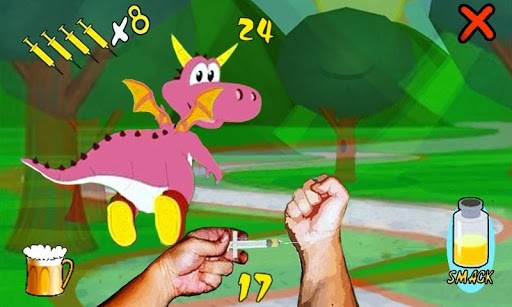
\includegraphics[width=4in]{HeroinHero.jpg}
\end{center}

\end{frame}

% -----------------------%%

\begin{frame}{Open Problem}\pause

\vspace{1em}

\begin{block}{\textbf{Comments} (continued)}

\vspace{-.5em}

\begin{itemize}
\item NAU undergraduate math and physics major \alert{Dustin Story} has been working on this problem all year. \pause
\item According to sequence \alert{A006245} of the OEIS, the first 10 values for $c_n$ (starting at $n=0$) are
\[
1, 1, 2, 8, 62, 908, 24698, 1232944, 112018190, 18410581880.
\]
\pause
\item To date, only the first 15 terms are known. \pause
\item The current best upper-bound for $c_n$ was obtained by Felsner and Valtr in 2011.  They prove that for sufficiently large $n$, $c_n\leq 2^{0.6571(n+1)^2}$. This bound is pretty awful.\pause
\item It turns out that the commutation classes of the longest element in $W(A_n)$ are in bijection with several interesting collections of mathematical objects. That is, $c_n$ counts other cool stuff.
\end{itemize}
\end{block}

\end{frame}

%% -----------------------%%

\begin{frame}{Heaps}\pause

\vspace{1em}

We now introduce \alert{heaps} through an example. \pause

\begin{block}{\textbf{Example}}

\vspace{-.5em}

Let $W$ be the Coxeter group of type $A_5$ and let $\overline{w} = s_1s_2s_3s_1s_2s_4s_5$ be a reduced expression for $w \in W$.

\vspace{-1em}

\begin{center}
\begin{tikzpicture}[scale=0.6]
\node at (-1.5,0.5) {$s_5$}; \node at (-1.5,1) {$s_4$}; \node at (-1.5,1.5) {$s_3$}; \node at (-1.5,2) {$s_2$}; \node at (-1.5,2.5) {$s_1$};
\draw[dotted, line width=0.5pt] (-1.2,0.5) -- (4.2,0.5);
\draw[dotted, line width=0.5pt] (-1.2,1)   -- (4.2,1);
\draw[dotted, line width=0.5pt] (-1.2,1.5) -- (4.2,1.5);
\draw[dotted, line width=0.5pt] (-1.2,2)   -- (4.2,2);
\draw[dotted, line width=0.5pt] (-1.2,2.5) -- (4.2,2.5); 
\pause
\sq{-1}{3};   \node at (-0.5,2.5) {$1$}; \pause
\sq{0}{2.5}; \node at (0.5,2)    {$2$}; \pause
\sq{1}{2}; \node at (1.5,1.5)    {$3$}; \pause
\sq{1}{3};   \node at (1.5,2.5)  {$1$}; \pause
\sq{2}{1.5};   \node at (2.5,1)  {$4$}; \pause
\sq{2}{2.5}; \node at (2.5,2)    {$2$}; \pause
\sq{3}{1};   \node at (3.5,.5)  {$5$};\pause
\end{tikzpicture}
\end{center}
\end{block}

\vspace{-1em}

\onslide<10->{Any element of the commutation class containing $\overline{w}$ has the heap above.}
\end{frame}

%% -----------------------%%

\begin{frame}{Heaps}\pause

\vspace{1em}

\begin{block}{\textbf{Theorem} (Stembridge)}

\vspace{-.5em}

There is a 1-1 correspondence between heaps and commutation classes.
\end{block}

\pause

\begin{block}{\textbf{Corollary}}

\vspace{-.5em}

The number of heaps for the longest element in $W(A_n)$ is $c_n$.
\end{block}

\pause

\begin{block}{\textbf{Example}}

\vspace{-.5em}

Here are the 8 heaps that correspond to the commutation classes for the longest element in $W(A_3)$.

\vspace{-1em}

\begin{center}
\begin{tabular}{llll}
\begin{tikzpicture}[scale=0.25]
\nsq{4}{3}{1}
\nsq{2}{2}{2}
\nsq{6}{2}{2}
\nsq{4}{1}{3}
\nsq{0}{1}{3}
\nsq{8}{1}{3}
\end{tikzpicture} \hspace{.2cm} &
\begin{tikzpicture}[scale=0.25]
\nsq{0}{3}{1}
\nsq{4}{3}{1}
\nsq{2}{2}{2}
\nsq{6}{2}{2}
\nsq{4}{1}{3}
\nsq{0}{1}{3}
\end{tikzpicture} \hspace{.2cm} &
\begin{tikzpicture}[scale=0.25]
\nsq{4}{3}{1}
\nsq{2}{2}{2}
\nsq{6}{2}{2}
\nsq{10}{2}{2}
\nsq{0}{1}{3}
\nsq{8}{1}{3}
\end{tikzpicture} \hspace{.2cm} &
\begin{tikzpicture}[scale=0.25]
\nsq{4}{3}{1}
\nsq{-2}{2}{2}
\nsq{2}{2}{2}
\nsq{6}{2}{2}
\nsq{0}{1}{3}
\nsq{8}{1}{3}
\end{tikzpicture} \\
\\
\begin{tikzpicture}[scale=0.25]
\nsq{4}{1}{3}
\nsq{2}{2}{2}
\nsq{6}{2}{2}
\nsq{4}{3}{1}
\nsq{0}{3}{1}
\nsq{8}{3}{1}
\end{tikzpicture} &
\begin{tikzpicture}[scale=0.25]
\nsq{0}{3}{1}
\nsq{4}{3}{1}
\nsq{2}{2}{2}
\nsq{-2}{2}{2}
\nsq{4}{1}{3}
\nsq{0}{1}{3}
\end{tikzpicture} &
\begin{tikzpicture}[scale=0.25]
\nsq{0}{3}{1}
\nsq{8}{3}{1}
\nsq{2}{2}{2}
\nsq{6}{2}{2}
\nsq{10}{2}{2}
\nsq{4}{1}{3}
\end{tikzpicture} &
\begin{tikzpicture}[scale=0.25]
\nsq{4}{1}{3}
\nsq{-2}{2}{2}
\nsq{2}{2}{2}
\nsq{6}{2}{2}
\nsq{0}{3}{1}
\nsq{8}{3}{1}
\end{tikzpicture}
\end{tabular}
\end{center}
  
\end{block}

\end{frame}

%% -----------------------%%

\begin{frame}{String Diagrams}\pause

\vspace{1em}

One way of representing permutations is via \alert{string diagrams}.

\pause

\begin{block}{\textbf{Example}}

\vspace{-.5em}

Consider $\sigma=(1,2,5,3)(4,6)$. 

\vspace{-1em}

\begin{center}
\begin{tikzpicture}[scale=.5]
\draw[fill=black] \foreach \y in {0,1,2,3,4,5} {(0,\y) circle (2pt)};
\draw[fill=black] \foreach \y in {0,1,2,3,4,5} {(6,\y) circle (2pt)};
\node at (0,0){%
\psset{unit=0.5cm}
\pscurve{-}(0,1)(1.5,1.5)(3,2.5)(6,3)
};
\node at (0,0){%
\psset{unit=0.5cm}
\pscurve{-}(0,0)(3,.5)(4.5,1.5)(6,2)
};
\node at (0,0){%
\psset{unit=0.5cm}
\pscurve{-}(0,2)(1.5,1.5)(3,.5)(6,0)
};
\node at (0,0){%
\psset{unit=0.5cm}
\pscurve{-}(0,4)(1.5,3.5)(3,2.5)(4.5,1.5)(6,1)
};
\node at (0,0){%
\psset{unit=0.5cm}
\pscurve{-}(0,5)(3,4.5)(6,4)
};
\node at (0,0){%
\psset{unit=0.5cm}
\pscurve{-}(0,3)(1.5,3.5)(3,4.5)(6,5)
};
\end{tikzpicture}
\end{center}

\end{block}

\vspace{-1em}

\pause

\begin{block}{\textbf{Comment}}

\vspace{-.5em}

When drawing a string diagram, we adopt the following conventions:

\vspace{-.5em}

\begin{itemize}
\item No more than two strings cross each other at a given point.
\item Strings are drawn to minimize crossings.
\end{itemize}
\end{block}

\end{frame}

%% -----------------------%%

\begin{frame}{String Diagrams}\pause

\vspace{1em}

One often has many choices about how the strings are drawn. Loosely speaking, we say that two string diagrams are \alert{equivalent} iff the relative arrangement of the crossings of the strings are the same.

\pause

\begin{block}{\textbf{Theorem}}

\vspace{-.5em}

Up to equivalence, there is a 1-1 correspondence between string diagrams for a permutation in $S_{n+1}$ and heaps for the corresponding permutation in $W(A_n)$. The points at which two strings cross correspond to blocks in a heap.
\end{block}

\pause

\begin{block}{\textbf{Example}}

\vspace{-1.5em}

\begin{center} 
\begin{tikzpicture}[scale=0.35]
\nsq{0}{0.5}{};
\nsq{0}{2.5}{};
\nsq{0}{4.5}{};
\nsq{2}{-.5}{};
\nsq{2}{1.5}{};
\nsq{2}{3.5}{};
\nsq{4}{0.5}{};
\nsq{4}{4.5}{};
\draw [purple,very thick] plot [smooth, tension=0.8] coordinates {(7,4)(5,3.5)(3,2.5)(1,1.5)(-1,1)};
\draw [purple,very thick] plot [smooth, tension=0.8] coordinates {(7,3)(5,3.5)(3,5.5)(1,3.5)(-1,3)};
\draw [purple,very thick] plot [smooth, tension=0.8] coordinates {(7,2)(5,1.8)(3,2.5)(1,3.5)(-1,4)};
\draw [purple,very thick] plot [smooth, tension=0.8] coordinates {(7,1)(5,1.02)(3,0.5)(1,-.5)(-1,-1)};
\draw [purple,very thick] plot [smooth, tension=0.8] coordinates {(7,0)(5,-.5)(3,-1.5)(1,-2.5)(-1,-2)};
\draw [purple,very thick] plot [smooth, tension=0.8] coordinates {(7,-1)(5,-.5)(3,0.5)(1,1.5)(-1,2)};
\draw [purple,very thick] plot [smooth, tension=0.8] coordinates {(7,-2)(5,-2.5)(3,-1.5)(1,-0.5)(-1,0)};
\draw[fill=black] \foreach \y in {-1,-2,0,1,2,3,4} {(7,\y) circle (3pt)};
\draw[fill=black] \foreach \y in {-1,-2,0,1,2,3,4} {(-1,\y) circle (3pt)};
\end{tikzpicture}
\end{center}

\end{block}

\end{frame}

%% -----------------------%%

\begin{frame}{String Diagrams}\pause

\vspace{1em}

\begin{block}{\textbf{Corollary}}

\vspace{-.5em}

The number of string diagrams (up to equivalence) for the longest element in $S_{n+1}$ is $c_n$.
\end{block}

\pause

\begin{block}{\textbf{Definition}}

\vspace{-.5em}

An \alert{arrangement of pseudolines} is a family of pseudolines with the property that each pair of pseudolines has a unique point of intersection. An arrangement is \alert{simple} if no three pseudolines have a common point of intersection.
\end{block}

\pause

\begin{block}{\textbf{Corollary}}

\vspace{-.5em}

The number of simple arrangements of $n+1$ pseudolines (up to equivalence) is $c_n$.
\end{block}

\end{frame}

%% -----------------------%%

\begin{frame}{Primitive Sorting Networks}\pause

\vspace{1em}

\begin{block}{\textbf{Definition}}

\vspace{-.5em}

A \alert{comparator} $[i : j]$ operates on a sequence of numbers $(x_1,\ldots, x_n)$ by replacing $x_i$ and $x_j$ respectively by $\min(x_i, x_j)$ and $\max(x_i, x_i)$. 

\pause

A \alert{sorting network} is a sequence of comparators that will sort any given sequence $(x_1,\ldots,x_n)$. That is, the successive comparators will produce an output sequence that always satisfies $x_1\leq\cdots \leq x_n$. A sorting network is called \alert{primitive} if its comparators all have the form $[i : i + 1]$.
\end{block}

\pause

\begin{block}{\textbf{Theorem}}

\vspace{-.5em}

A sequence of comparators is a sorting network iff it sorts the single permutation $[n,..., 2, 1]$.  A minimal primitive sorting network is equivalent to a sequence of adjacent transpositions $(i,i + 1)$ that changes a sequence $(x_1, x_2,\ldots ,x_n)$ into its reflection $(x_n,\ldots, x_2, x_1)$.

\end{block}

\end{frame}

%% -----------------------%%

\begin{frame}{Primitive Sorting Networks}\pause

\vspace{1em}

Primitive sorting networks can be represented with \alert{ladder diagrams} (also called \alert{ladder lotteries}, \alert{Amidakuji}, or \alert{ghost legs}).

\pause

\begin{block}{\textbf{Example}}

\vspace{-.5em}

Here are the minimal ladder diagrams that correspond to the 8 primitive sorting networks on 4 elements.

\vspace{-.5em}

\begin{center}
\begin{tabular}{llll}
\begin{tikzpicture}[scale=0.4]
\draw[very thick] (0,0) -- (6,0);
\draw[very thick] (0,1) -- (6,1);
\draw[very thick] (0,2) -- (6,2);
\draw[very thick] (0,3) -- (6,3);
\draw[very thick] (1,0) -- (1,1);
\draw[very thick] (3,0) -- (3,1);
\draw[very thick] (5,0) -- (5,1);
\draw[very thick] (2,1) -- (2,2);
\draw[very thick] (4,1) -- (4,2);
\draw[very thick] (3,2) -- (3,3);
\end{tikzpicture} \hspace{.3cm} &
\begin{tikzpicture}[scale=0.4]
\draw[very thick] (0,0) -- (5,0);
\draw[very thick] (0,1) -- (5,1);
\draw[very thick] (0,2) -- (5,2);
\draw[very thick] (0,3) -- (5,3);
\draw[very thick] (1,0) -- (1,1);
\draw[very thick] (3,0) -- (3,1);
\draw[very thick] (1,2) -- (1,3);
\draw[very thick] (2,1) -- (2,2);
\draw[very thick] (4,1) -- (4,2);
\draw[very thick] (3,2) -- (3,3);
\end{tikzpicture} \hspace{.3cm} &
\begin{tikzpicture}[scale=0.4]
\draw[very thick] (0,0) -- (7,0);
\draw[very thick] (0,1) -- (7,1);
\draw[very thick] (0,2) -- (7,2);
\draw[very thick] (0,3) -- (7,3);
\draw[very thick] (1,0) -- (1,1);
\draw[very thick] (6,1) -- (6,2);
\draw[very thick] (5,0) -- (5,1);
\draw[very thick] (2,1) -- (2,2);
\draw[very thick] (4,1) -- (4,2);
\draw[very thick] (3,2) -- (3,3);
\end{tikzpicture} \hspace{.3cm} &
\begin{tikzpicture}[scale=0.4]
\draw[very thick] (0,0) -- (7,0);
\draw[very thick] (0,1) -- (7,1);
\draw[very thick] (0,2) -- (7,2);
\draw[very thick] (0,3) -- (7,3);
\draw[very thick] (2,0) -- (2,1);
\draw[very thick] (1,1) -- (1,2);
\draw[very thick] (6,0) -- (6,1);
\draw[very thick] (3,1) -- (3,2);
\draw[very thick] (5,1) -- (5,2);
\draw[very thick] (4,2) -- (4,3);
\end{tikzpicture} \\
\\
\begin{tikzpicture}[scale=0.4]
\draw[very thick] (0,0) -- (6,0);
\draw[very thick] (0,1) -- (6,1);
\draw[very thick] (0,2) -- (6,2);
\draw[very thick] (0,3) -- (6,3);
\draw[very thick] (1,2) -- (1,3);
\draw[very thick] (3,2) -- (3,3);
\draw[very thick] (5,2) -- (5,3);
\draw[very thick] (2,1) -- (2,2);
\draw[very thick] (4,1) -- (4,2);
\draw[very thick] (3,0) -- (3,1);
\end{tikzpicture} &
\begin{tikzpicture}[scale=0.4]
\draw[very thick] (0,0) -- (5,0);
\draw[very thick] (0,1) -- (5,1);
\draw[very thick] (0,2) -- (5,2);
\draw[very thick] (0,3) -- (5,3);
\draw[very thick] (2,0) -- (2,1);
\draw[very thick] (4,0) -- (4,1);
\draw[very thick] (2,2) -- (2,3);
\draw[very thick] (3,1) -- (3,2);
\draw[very thick] (1,1) -- (1,2);
\draw[very thick] (4,2) -- (4,3);
\end{tikzpicture} &
\begin{tikzpicture}[scale=0.4]
\draw[very thick] (0,0) -- (7,0);
\draw[very thick] (0,1) -- (7,1);
\draw[very thick] (0,2) -- (7,2);
\draw[very thick] (0,3) -- (7,3);
\draw[very thick] (1,2) -- (1,3);
\draw[very thick] (6,1) -- (6,2);
\draw[very thick] (5,2) -- (5,3);
\draw[very thick] (2,1) -- (2,2);
\draw[very thick] (4,1) -- (4,2);
\draw[very thick] (3,0) -- (3,1);
\end{tikzpicture} &
\begin{tikzpicture}[scale=0.4]
\draw[very thick] (0,0) -- (7,0);
\draw[very thick] (0,1) -- (7,1);
\draw[very thick] (0,2) -- (7,2);
\draw[very thick] (0,3) -- (7,3);
\draw[very thick] (2,2) -- (2,3);
\draw[very thick] (1,1) -- (1,2);
\draw[very thick] (6,2) -- (6,3);
\draw[very thick] (3,1) -- (3,2);
\draw[very thick] (5,1) -- (5,2);
\draw[very thick] (4,0) -- (4,1);
\end{tikzpicture}
\end{tabular}
\end{center}

\end{block}

\end{frame}

%% -----------------------%%

\begin{frame}{Primitive Sorting Networks}\pause

\vspace{1em}

\begin{block}{\textbf{Theorem}}

\vspace{-.5em}

There is a 1-1 correspondence between minimal primitive sorting networks on $n+1$ elements and heaps of the longest element in $W(A_n)$. Each rung in a ladder corresponds to a block in the heap.
\end{block}

\pause

\begin{block}{\textbf{Corollary}}

\vspace{-.5em}

The number of minimal primitive sorting networks on $n+1$ elements is $c_n$.
\end{block}

\end{frame}

%% -----------------------%%

\begin{frame}{Rhombic Tilings}\pause

\vspace{1em}

It turns out that you can always tile a regular $2k$-gon using rhombi such that all side lengths of the rhombi and the $2k$-gon are the same.

\pause

\begin{block}{\textbf{Example}}

\vspace{-.5em}

Here are the 8 distinct rhombic tilings of a regular octagon.

\vspace{-1em}

\begin{center}
\begin{tabular}{llllllll}
\begin{tikzpicture}[scale=.28]
\draw [color=black] (1.0447355787000123,0.)-- (-0.6428174477092435,0.6928452343127731);
\draw [color=black] (-0.6428174477092435,0.6928452343127731)-- (-2.326013199790454,-0.010519390777748772);
\draw [color=black] (-2.326013199790454,-0.010519390777748772)-- (-3.018858434103227,-1.6980724171870047);
\draw [color=black] (-3.018858434103227,-1.6980724171870047)-- (-2.3154938090127053,-3.381268169268215);
\draw [color=black] (-2.3154938090127053,-3.381268169268215)-- (-0.6279407826034493,-4.074113403580988);
\draw [color=black] (-0.6279407826034493,-4.074113403580988)-- (1.0552549694777609,-3.3707487784904666);
\draw [color=black] (1.0552549694777609,-3.3707487784904666)-- (1.7481002037905344,-1.6831957520812106);
\draw [color=black] (1.7481002037905344,-1.6831957520812106)-- (1.0447355787000123,0.);
\draw (-2.326013199790454,-0.010519390777748772)-- (-0.6428174477092435,0.6928452343127731);
\draw (-2.326013199790454,-0.010519390777748772)-- (-0.6384601733811982,-0.7033646250905218);
\draw (-0.6384601733811982,-0.7033646250905218)-- (1.0447355787000123,0.);
\draw (-0.6384601733811982,-0.7033646250905218)-- (-1.3313054076939714,-2.390917651499778);
\draw (-3.018858434103227,-1.6980724171870047)-- (-1.3313054076939714,-2.390917651499778);
\draw (-1.3313054076939714,-2.390917651499778)-- (-0.6279407826034493,-4.074113403580988);
\draw (-0.6279407826034493,-4.074113403580988)-- (0.06490445170932387,-2.3865603771717327);
\draw (0.06490445170932387,-2.3865603771717327)-- (1.7481002037905344,-1.6831957520812106);
\draw (0.06490445170932387,-2.3865603771717327)-- (-0.6384601733811982,-0.7033646250905218);
\draw (-3.018858434103227,-1.6980724171870047)-- (-1.3313054076939714,-2.390917651499778);
\end{tikzpicture}  &
\begin{tikzpicture}[scale=.28]
\begin{scope}[rotate=270]
\draw [color=black] (1.0447355787000123,0.)-- (-0.6428174477092435,0.6928452343127731);
\draw [color=black] (-0.6428174477092435,0.6928452343127731)-- (-2.326013199790454,-0.010519390777748772);
\draw [color=black] (-2.326013199790454,-0.010519390777748772)-- (-3.018858434103227,-1.6980724171870047);
\draw [color=black] (-3.018858434103227,-1.6980724171870047)-- (-2.3154938090127053,-3.381268169268215);
\draw [color=black] (-2.3154938090127053,-3.381268169268215)-- (-0.6279407826034493,-4.074113403580988);
\draw [color=black] (-0.6279407826034493,-4.074113403580988)-- (1.0552549694777609,-3.3707487784904666);
\draw [color=black] (1.0552549694777609,-3.3707487784904666)-- (1.7481002037905344,-1.6831957520812106);
\draw [color=black] (1.7481002037905344,-1.6831957520812106)-- (1.0447355787000123,0.);
\draw (-2.326013199790454,-0.010519390777748772)-- (-0.6428174477092435,0.6928452343127731);
\draw (-2.326013199790454,-0.010519390777748772)-- (-0.6384601733811982,-0.7033646250905218);
\draw (-0.6384601733811982,-0.7033646250905218)-- (1.0447355787000123,0.);
\draw (-0.6384601733811982,-0.7033646250905218)-- (-1.3313054076939714,-2.390917651499778);
\draw (-3.018858434103227,-1.6980724171870047)-- (-1.3313054076939714,-2.390917651499778);
\draw (-1.3313054076939714,-2.390917651499778)-- (-0.6279407826034493,-4.074113403580988);
\draw (-0.6279407826034493,-4.074113403580988)-- (0.06490445170932387,-2.3865603771717327);
\draw (0.06490445170932387,-2.3865603771717327)-- (1.7481002037905344,-1.6831957520812106);
\draw (0.06490445170932387,-2.3865603771717327)-- (-0.6384601733811982,-0.7033646250905218);
\draw (-3.018858434103227,-1.6980724171870047)-- (-1.3313054076939714,-2.390917651499778);
\end{scope}
\end{tikzpicture}  &
\begin{tikzpicture}[scale=.28]
\begin{scope}[rotate=135]
\draw [color=black] (1.0447355787000123,0.)-- (-0.6428174477092435,0.6928452343127731);
\draw [color=black] (-0.6428174477092435,0.6928452343127731)-- (-2.326013199790454,-0.010519390777748772);
\draw [color=black] (-2.326013199790454,-0.010519390777748772)-- (-3.018858434103227,-1.6980724171870047);
\draw [color=black] (-3.018858434103227,-1.6980724171870047)-- (-2.3154938090127053,-3.381268169268215);
\draw [color=black] (-2.3154938090127053,-3.381268169268215)-- (-0.6279407826034493,-4.074113403580988);
\draw [color=black] (-0.6279407826034493,-4.074113403580988)-- (1.0552549694777609,-3.3707487784904666);
\draw [color=black] (1.0552549694777609,-3.3707487784904666)-- (1.7481002037905344,-1.6831957520812106);
\draw [color=black] (1.7481002037905344,-1.6831957520812106)-- (1.0447355787000123,0.);
\draw (-2.326013199790454,-0.010519390777748772)-- (-0.6428174477092435,0.6928452343127731);
\draw (-2.326013199790454,-0.010519390777748772)-- (-0.6384601733811982,-0.7033646250905218);
\draw (-0.6384601733811982,-0.7033646250905218)-- (1.0447355787000123,0.);
\draw (-0.6384601733811982,-0.7033646250905218)-- (-1.3313054076939714,-2.390917651499778);
\draw (-3.018858434103227,-1.6980724171870047)-- (-1.3313054076939714,-2.390917651499778);
\draw (-1.3313054076939714,-2.390917651499778)-- (-0.6279407826034493,-4.074113403580988);
\draw (-0.6279407826034493,-4.074113403580988)-- (0.06490445170932387,-2.3865603771717327);
\draw (0.06490445170932387,-2.3865603771717327)-- (1.7481002037905344,-1.6831957520812106);
\draw (0.06490445170932387,-2.3865603771717327)-- (-0.6384601733811982,-0.7033646250905218);
\draw (-3.018858434103227,-1.6980724171870047)-- (-1.3313054076939714,-2.390917651499778);
\end{scope}
\end{tikzpicture}  &
\begin{tikzpicture}[scale=.28]
\begin{scope}[rotate=225]
\draw [color=black] (1.0447355787000123,0.)-- (-0.6428174477092435,0.6928452343127731);
\draw [color=black] (-0.6428174477092435,0.6928452343127731)-- (-2.326013199790454,-0.010519390777748772);
\draw [color=black] (-2.326013199790454,-0.010519390777748772)-- (-3.018858434103227,-1.6980724171870047);
\draw [color=black] (-3.018858434103227,-1.6980724171870047)-- (-2.3154938090127053,-3.381268169268215);
\draw [color=black] (-2.3154938090127053,-3.381268169268215)-- (-0.6279407826034493,-4.074113403580988);
\draw [color=black] (-0.6279407826034493,-4.074113403580988)-- (1.0552549694777609,-3.3707487784904666);
\draw [color=black] (1.0552549694777609,-3.3707487784904666)-- (1.7481002037905344,-1.6831957520812106);
\draw [color=black] (1.7481002037905344,-1.6831957520812106)-- (1.0447355787000123,0.);
\draw (-2.326013199790454,-0.010519390777748772)-- (-0.6428174477092435,0.6928452343127731);
\draw (-2.326013199790454,-0.010519390777748772)-- (-0.6384601733811982,-0.7033646250905218);
\draw (-0.6384601733811982,-0.7033646250905218)-- (1.0447355787000123,0.);
\draw (-0.6384601733811982,-0.7033646250905218)-- (-1.3313054076939714,-2.390917651499778);
\draw (-3.018858434103227,-1.6980724171870047)-- (-1.3313054076939714,-2.390917651499778);
\draw (-1.3313054076939714,-2.390917651499778)-- (-0.6279407826034493,-4.074113403580988);
\draw (-0.6279407826034493,-4.074113403580988)-- (0.06490445170932387,-2.3865603771717327);
\draw (0.06490445170932387,-2.3865603771717327)-- (1.7481002037905344,-1.6831957520812106);
\draw (0.06490445170932387,-2.3865603771717327)-- (-0.6384601733811982,-0.7033646250905218);
\draw (-3.018858434103227,-1.6980724171870047)-- (-1.3313054076939714,-2.390917651499778);
\end{scope}
\end{tikzpicture}  &
\begin{tikzpicture}[scale=.28]
\begin{scope}[rotate=180]
\draw [color=black] (1.0447355787000123,0.)-- (-0.6428174477092435,0.6928452343127731);
\draw [color=black] (-0.6428174477092435,0.6928452343127731)-- (-2.326013199790454,-0.010519390777748772);
\draw [color=black] (-2.326013199790454,-0.010519390777748772)-- (-3.018858434103227,-1.6980724171870047);
\draw [color=black] (-3.018858434103227,-1.6980724171870047)-- (-2.3154938090127053,-3.381268169268215);
\draw [color=black] (-2.3154938090127053,-3.381268169268215)-- (-0.6279407826034493,-4.074113403580988);
\draw [color=black] (-0.6279407826034493,-4.074113403580988)-- (1.0552549694777609,-3.3707487784904666);
\draw [color=black] (1.0552549694777609,-3.3707487784904666)-- (1.7481002037905344,-1.6831957520812106);
\draw [color=black] (1.7481002037905344,-1.6831957520812106)-- (1.0447355787000123,0.);
\draw (-2.326013199790454,-0.010519390777748772)-- (-0.6428174477092435,0.6928452343127731);
\draw (-2.326013199790454,-0.010519390777748772)-- (-0.6384601733811982,-0.7033646250905218);
\draw (-0.6384601733811982,-0.7033646250905218)-- (1.0447355787000123,0.);
\draw (-0.6384601733811982,-0.7033646250905218)-- (-1.3313054076939714,-2.390917651499778);
\draw (-3.018858434103227,-1.6980724171870047)-- (-1.3313054076939714,-2.390917651499778);
\draw (-1.3313054076939714,-2.390917651499778)-- (-0.6279407826034493,-4.074113403580988);
\draw (-0.6279407826034493,-4.074113403580988)-- (0.06490445170932387,-2.3865603771717327);
\draw (0.06490445170932387,-2.3865603771717327)-- (1.7481002037905344,-1.6831957520812106);
\draw (0.06490445170932387,-2.3865603771717327)-- (-0.6384601733811982,-0.7033646250905218);
\draw (-3.018858434103227,-1.6980724171870047)-- (-1.3313054076939714,-2.390917651499778);
\end{scope}
\end{tikzpicture}  &
\begin{tikzpicture}[scale=.28]
\begin{scope}[rotate=90]
\draw [color=black] (1.0447355787000123,0.)-- (-0.6428174477092435,0.6928452343127731);
\draw [color=black] (-0.6428174477092435,0.6928452343127731)-- (-2.326013199790454,-0.010519390777748772);
\draw [color=black] (-2.326013199790454,-0.010519390777748772)-- (-3.018858434103227,-1.6980724171870047);
\draw [color=black] (-3.018858434103227,-1.6980724171870047)-- (-2.3154938090127053,-3.381268169268215);
\draw [color=black] (-2.3154938090127053,-3.381268169268215)-- (-0.6279407826034493,-4.074113403580988);
\draw [color=black] (-0.6279407826034493,-4.074113403580988)-- (1.0552549694777609,-3.3707487784904666);
\draw [color=black] (1.0552549694777609,-3.3707487784904666)-- (1.7481002037905344,-1.6831957520812106);
\draw [color=black] (1.7481002037905344,-1.6831957520812106)-- (1.0447355787000123,0.);
\draw (-2.326013199790454,-0.010519390777748772)-- (-0.6428174477092435,0.6928452343127731);
\draw (-2.326013199790454,-0.010519390777748772)-- (-0.6384601733811982,-0.7033646250905218);
\draw (-0.6384601733811982,-0.7033646250905218)-- (1.0447355787000123,0.);
\draw (-0.6384601733811982,-0.7033646250905218)-- (-1.3313054076939714,-2.390917651499778);
\draw (-3.018858434103227,-1.6980724171870047)-- (-1.3313054076939714,-2.390917651499778);
\draw (-1.3313054076939714,-2.390917651499778)-- (-0.6279407826034493,-4.074113403580988);
\draw (-0.6279407826034493,-4.074113403580988)-- (0.06490445170932387,-2.3865603771717327);
\draw (0.06490445170932387,-2.3865603771717327)-- (1.7481002037905344,-1.6831957520812106);
\draw (0.06490445170932387,-2.3865603771717327)-- (-0.6384601733811982,-0.7033646250905218);
\draw (-3.018858434103227,-1.6980724171870047)-- (-1.3313054076939714,-2.390917651499778);
\end{scope}
\end{tikzpicture}  &
\begin{tikzpicture}[scale=.28]
\begin{scope}[rotate=45]
\draw [color=black] (1.0447355787000123,0.)-- (-0.6428174477092435,0.6928452343127731);
\draw [color=black] (-0.6428174477092435,0.6928452343127731)-- (-2.326013199790454,-0.010519390777748772);
\draw [color=black] (-2.326013199790454,-0.010519390777748772)-- (-3.018858434103227,-1.6980724171870047);
\draw [color=black] (-3.018858434103227,-1.6980724171870047)-- (-2.3154938090127053,-3.381268169268215);
\draw [color=black] (-2.3154938090127053,-3.381268169268215)-- (-0.6279407826034493,-4.074113403580988);
\draw [color=black] (-0.6279407826034493,-4.074113403580988)-- (1.0552549694777609,-3.3707487784904666);
\draw [color=black] (1.0552549694777609,-3.3707487784904666)-- (1.7481002037905344,-1.6831957520812106);
\draw [color=black] (1.7481002037905344,-1.6831957520812106)-- (1.0447355787000123,0.);
\draw (-2.326013199790454,-0.010519390777748772)-- (-0.6428174477092435,0.6928452343127731);
\draw (-2.326013199790454,-0.010519390777748772)-- (-0.6384601733811982,-0.7033646250905218);
\draw (-0.6384601733811982,-0.7033646250905218)-- (1.0447355787000123,0.);
\draw (-0.6384601733811982,-0.7033646250905218)-- (-1.3313054076939714,-2.390917651499778);
\draw (-3.018858434103227,-1.6980724171870047)-- (-1.3313054076939714,-2.390917651499778);
\draw (-1.3313054076939714,-2.390917651499778)-- (-0.6279407826034493,-4.074113403580988);
\draw (-0.6279407826034493,-4.074113403580988)-- (0.06490445170932387,-2.3865603771717327);
\draw (0.06490445170932387,-2.3865603771717327)-- (1.7481002037905344,-1.6831957520812106);
\draw (0.06490445170932387,-2.3865603771717327)-- (-0.6384601733811982,-0.7033646250905218);
\draw (-3.018858434103227,-1.6980724171870047)-- (-1.3313054076939714,-2.390917651499778);
\end{scope}
\end{tikzpicture}  &
\begin{tikzpicture}[scale=.28]
\begin{scope}[rotate=315]
\draw [color=black] (1.0447355787000123,0.)-- (-0.6428174477092435,0.6928452343127731);
\draw [color=black] (-0.6428174477092435,0.6928452343127731)-- (-2.326013199790454,-0.010519390777748772);
\draw [color=black] (-2.326013199790454,-0.010519390777748772)-- (-3.018858434103227,-1.6980724171870047);
\draw [color=black] (-3.018858434103227,-1.6980724171870047)-- (-2.3154938090127053,-3.381268169268215);
\draw [color=black] (-2.3154938090127053,-3.381268169268215)-- (-0.6279407826034493,-4.074113403580988);
\draw [color=black] (-0.6279407826034493,-4.074113403580988)-- (1.0552549694777609,-3.3707487784904666);
\draw [color=black] (1.0552549694777609,-3.3707487784904666)-- (1.7481002037905344,-1.6831957520812106);
\draw [color=black] (1.7481002037905344,-1.6831957520812106)-- (1.0447355787000123,0.);
\draw (-2.326013199790454,-0.010519390777748772)-- (-0.6428174477092435,0.6928452343127731);
\draw (-2.326013199790454,-0.010519390777748772)-- (-0.6384601733811982,-0.7033646250905218);
\draw (-0.6384601733811982,-0.7033646250905218)-- (1.0447355787000123,0.);
\draw (-0.6384601733811982,-0.7033646250905218)-- (-1.3313054076939714,-2.390917651499778);
\draw (-3.018858434103227,-1.6980724171870047)-- (-1.3313054076939714,-2.390917651499778);
\draw (-1.3313054076939714,-2.390917651499778)-- (-0.6279407826034493,-4.074113403580988);
\draw (-0.6279407826034493,-4.074113403580988)-- (0.06490445170932387,-2.3865603771717327);
\draw (0.06490445170932387,-2.3865603771717327)-- (1.7481002037905344,-1.6831957520812106);
\draw (0.06490445170932387,-2.3865603771717327)-- (-0.6384601733811982,-0.7033646250905218);
\draw (-3.018858434103227,-1.6980724171870047)-- (-1.3313054076939714,-2.390917651499778);
\end{scope}
\end{tikzpicture}
\end{tabular}
\end{center}

\pause

\vspace{-1em}

In this case, all rhombic tilings are rotation equivalent, but this is far from true in general.

\end{block}

\end{frame}

%% -----------------------%%

\begin{frame}{Rhombic Tilings}\pause

\vspace{1em}

By now, I'm sure you've seen this coming$\ldots$

\pause

\begin{block}{\textbf{Theorem}}

\vspace{-.5em}

There is a 1-1 correspondence between rhombic tilings of a regular $2(n+1)$-gon and heaps of the longest element in $W(A_n)$. Each tile corresponds to a block in the heap.

\end{block}

\pause

\begin{block}{\textbf{Corollary}}

\vspace{-.5em}

The number of rhombic tilings of a regular $2(n+1)$-gon is $c_n$.
\end{block}

\end{frame}

%% -----------------------%%

\begin{frame}{Other Bijections}\pause

\vspace{1em}

\begin{block}{\textbf{But there's more!}}

\vspace{-.5em}

The number of commutation classes of the longest element is also related to the following. \pause

\vspace{-.5em}

\begin{itemize}

\item Uniform oriented matroids of rank 3. \pause
\item Condorcet domains (voting theory). \pause
\item Something about stability of quasicrystals (physics).
\end{itemize}
\end{block}

\end{frame}

%% -----------------------%%

\begin{frame}{Attempts to find a new upper bound}\pause

\vspace{1em}

This academic year, Dustin and I have been working on attaining an improved upper bound for $c_n$.  Our approach:

\pause

\vspace{-.5em}

\begin{itemize}
\item We can obtain all possible string diagrams on $n+1$ strings by inserting a new string in all possible ways (up to equivalence) for every string diagram on $n$ strings. \pause
\item In heap land, this is equivalent to ``splitting" and ``shifting" all the heaps for the longest element in $W(A_{n-1})$ and inserting a staircase of $n$ blocks. This really will yield all the heaps for the longest element in $W(A_n)$. \pause
\item It turns out that our idea is related to \alert{cut paths}. \pause
\item Strategy: Find a heap in $W(A_{n-1})$ with the greatest number of cut paths, count the cut paths, then multiply this number by the number of heaps of the longest element in $W(A_{n-1})$.
\end{itemize}

\end{frame}

%% -----------------------%%

\begin{frame}{Attempts to find a new upper bound}\pause

\vspace{1em}

\begin{itemize}

\item Obvious answer: The even-odd sorting network (aka, brick sort) has the most cut paths of any other heap. Thanks to Nandor, we discovered a sequence on OEIS that turned us onto a paper by Galambos and Reiner that contains a nice formula that clearly counts what we wanted. They conjectured the same thing we did. Sweet! \pause
\item Our proposed upper bound kicks the crap out of the current best known. We're gonna be famous! {\Large \alert{\textbf{\smiley{}}}} \pause
\item The problem is that our approach doesn't work. {\Large \alert{\textbf{\frownie{}}}} \pause
\item It turns out that the even-odd network/heap doesn't have the greatest number of cut paths, which is a bit baffling. \pause
\item Danilov, Karzanov, and Koshevoy constructed a counterexample in $S_{42}$, which simultaneously disproved conjectures by Fishburn, by Monjardet, and by Galambos and Reiner.
\end{itemize}

\vspace{-.5em} \pause

\begin{center}
OK, back to the drawing board.
\end{center}

\end{frame}

%% -----------------------%%

\end{document}

Todo:

- Mention help from Nandor, OEIS, Reiner paper, etc.
